% !TEX root = ../main.tex
\section{DARE: Dimension-Adaptive Reconfigurable Engine}
\label{sec:hardware}

\subsection{Architecture and Mode Control}
Fig.~\ref{fig:dare_arch} locates the adaptive mechanisms in the accelerator. At the top level [Fig.~\ref{fig:dare_arch}(a)], DDR traffic is staged through local PEA/VCU SRAMs and dispatched to a shared $36\times36$ INT8 PEA and a 36-MAC FP16 VCU. DARE adds no separate temporal engine; it specializes address generation, lane ownership, replay, and reduction control around the shared PEA.

Fig.~\ref{fig:dare_arch}(b) shows the control path. Existing GEMM fields configure the QACT AGU/Q Router, $4\times9$ Lane Mapper, and Weight/K/V AGU + Replay. Standard mode bypasses these controls. Temporal $QK^{\mathsf T}$ changes lane ownership, whereas temporal $PV$ activates tagged reduction, persistent accumulation, and deferred writeback. Fig.~\ref{fig:dare_arch}(c) shows that the VCU remains unchanged because DARE restores conventional contiguous interfaces before handoff.

\subsection{Shared-PEA Dataflows}

\begin{figure}[!t]
  \centering
  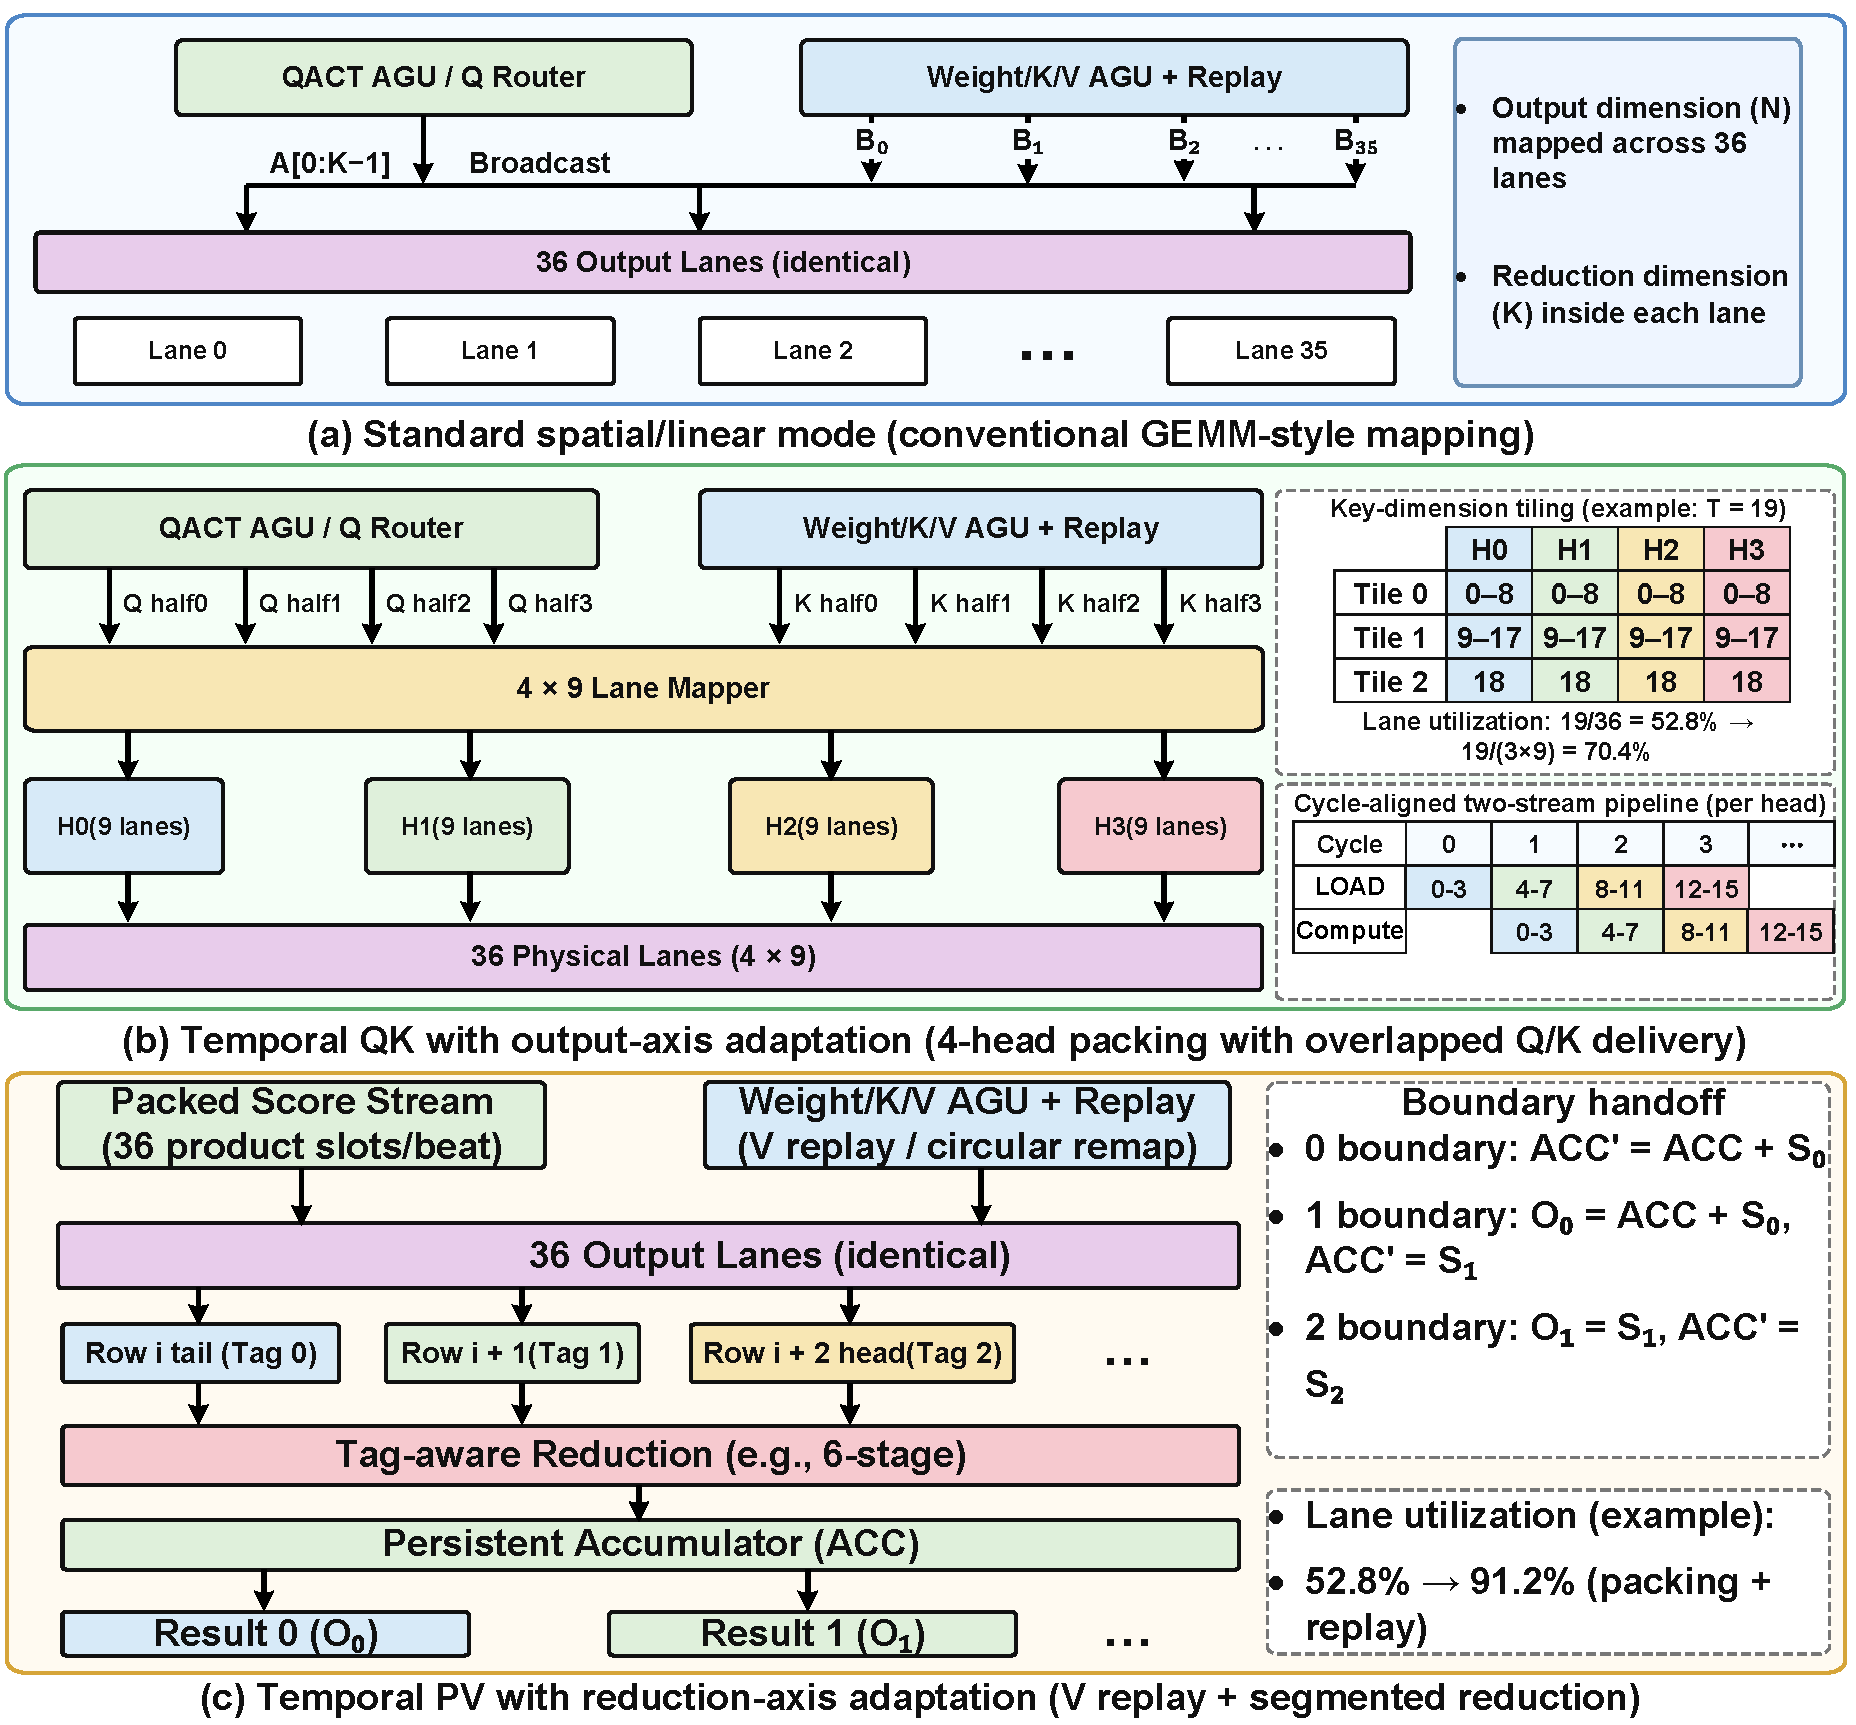
\includegraphics[width=\columnwidth]{fig/pea.pdf}
  \caption{Adaptive dataflows of the shared PEA: (a) conventional spatial/linear mapping; (b) temporal $QK^{\mathsf T}$ uses four 9-lane head groups; and (c) temporal $PV$ packs adjacent reductions with V replay and tagged segmented reduction.}
  \label{fig:dare_modes}
\end{figure}



Fig.~\ref{fig:dare_modes}(a) shows the conventional mapping: output dimension $N$ spans 36 lanes and reduction dimension $K$ is accumulated inside each lane. DARE preserves this interface and remaps only the temporal dimension when it becomes inefficient on either axis.

\subsection{Output-Axis Adaptation for $QK^{\mathsf T}$}
Temporal $QK^{\mathsf T}$ places sequence length on the output axis. With one head owning all 36 lanes, $T=19$ uses only $19/36=52.8\%$ of them. In Fig.~\ref{fig:dare_modes}(b), the $4\times9$ mapper partitions the PEA into four head groups H0--H3, each consuming nine key positions per tile while Q/K delivery overlaps. Three tiles cover positions 0--18, raising useful occupancy to $19/27=70.4\%$; longer sequences iterate the same tiled mapping. Completed dot products are drained in conventional order, preserving the downstream interface.

\subsection{Reduction-Axis Adaptation for $PV$}
In $PV$, the temporal dimension moves to the reduction axis, so DARE switches from lane partitioning to boundary-aware packing [Fig.~\ref{fig:dare_modes}(c)]. Products from adjacent rows share one 36-product beat; V entries are replayed to matching slots, and row tags prevent cross-row accumulation. A persistent accumulator carries a row across beats, while dual-result writeback handles beats that finish two rows without duplicating the reduction array or OFMAP SRAM port.

For $T=19$, one head contains $19^2=361$ products. Row padding uses only 19 of 36 slots per beat (52.8\%), whereas packed execution needs 11 beats, giving $361/(11\times36)=91.2\%$ useful-product occupancy. Thus Fig.~\ref{fig:dare_modes}(b) and (c) capture the DARE principle: the same PEA switches between output-axis remapping and reduction-axis packing as the variable dimension moves across the two attention GEMMs.
